\section{Modelli di programmazione parallela}
Esistono diversi modelli di programmazione parallela comunemente usati come la \textbf{memoria condivisa}, le \textbf{threads}, il \textbf{passaggio di messaggi}, il \textbf{parallelismo dei dati} e un approccio \textbf{ibrido}. Questi modelli sono un astrazione dell'hardware e delle architetture di memoria sottostanti.

Questi modelli non sono specifici di una particolare macchina o architettura di memoria. In effetti, ciascuno di questi modelli può essere implementato su qualsiasi hardware sottostante. Due esempi:
\begin{enumerate}
	\item modello di memoria condivisa su una memoria distribuita: approccio KSR (\textit{Kendall Square Research}) ALLCACHE. La memoria della macchina era distribuita fisicamente, ma appariva all'utente come un'unica memoria condivisa (spazio di indirizzi globale). Genericamente questo approccio viene definito come \textit{"macchina virtuale condivisa"};
	\item modello di passaggio del messaggio su una macchina con memoria condivisa. MPI su SGI Origin. SGI Origin utilizzava un'architettura di memoria condivisa di tipo CC-NUMA, in cui ogni attività ha accesso diretto alla memoria globale. Tuttavia, la capacità di inviare e ricevere messaggi con MPI, come avviene comunemente su una rete di macchine a memoria distribuita, non solo è implementata ma è utilizzata molto comunemente.
\end{enumerate}

Quale modello utilizzare è spesso una combinazione di ciò che è disponibile e di una scelta personale. Non esiste un modello "migliore", anche se esistono certamente implementazioni migliori di alcuni modelli rispetto ad altri.

\subsection{Modello di memoria condivisa} Nel modello di programmazione a memoria condivisa, le attività condividono uno spazio di indirizzi comune, che leggono e scrivono in modo asincrono. Vari meccanismi come lock o semafori possono essere utilizzati per controllare l'accesso alla memoria condivisa. Un vantaggio di questo modello dal punto di vista del programmatore è che manca la nozione di "proprietà" dei dati. Infatti non è necessario specificare esplicitamente la comunicazione dei dati tra le attività. Lo sviluppo del programma può essere semplificato. Uno svantaggio importante in termini di prestazioni è che diventa difficile comprendere e gestire la località dei dati. In effetti, risulta necessario mantenere i dati locali rispetto al processore che li utilizza, preserva gli accessi alla memoria, gli aggiornamenti della cache e il traffico del bus che si verifica quando più processori utilizzano gli stessi dati.

\subsubsection{Implementazione del modello di memoria condivisa} Sulle piattaforme di memoria condivisa, i compilatori nativi traducono variabili del programma utente in indirizzi di memoria effettivi, che sono globali. Attualmente non esistono implementazioni comuni della piattaforma di memoria distribuita. Tuttavia, l'approccio KSR ALLCACHE forniva una visualizzazione della memoria condivisa dei dati anche se la memoria fisica della macchina era distribuita.
\subsection{Modello con le thread}
\begin{figure}[th]
	\centering
	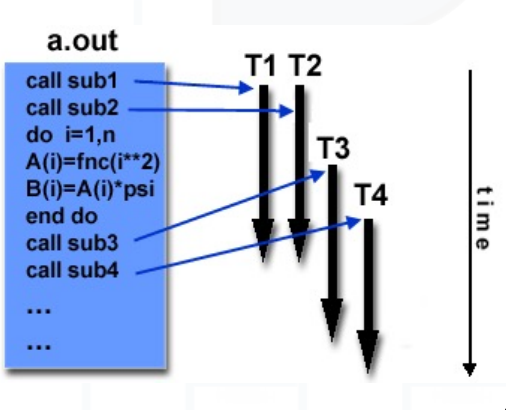
\includegraphics[width=0.7\linewidth]{img/modello-thread}
	\caption{modello con le thread.}
	\label{fig:modello-thread}
\end{figure}
Nel modello con le thread della programmazione parallela (figura \ref{fig:modello-thread}), un singolo processo può avere più percorsi di esecuzione simultanei. Forse l'analogia più semplice che può essere utilizzata per descrivere le thread, è il concetto di un singolo programma che include un numero di subroutine.
\begin{itemize}
	\item il programma principale a.out è pianificato per l'esecuzione dal sistema operativo. a.out carica ed acquisisce tutte le risorse utente e di sistema necessarie per l'esecuzione;
	\item a.out esegue del lavoro seriale e quindi crea una serie di thread che possono essere pianificate ed eseguite contemporaneamente dal sistema operativo;
	\item ogni thread ha dati locali, ma condivide anche tutte le risorse di a.out. Ciò consente di risparmiare il sovraccarico associato alla replica delle risorse di un programma per ciascuna thread. Ogni thread beneficia anche di una vista globale della memoria perché condivide lo spazio di memoria di a.out;
	\item il lavoro di una thread può essere meglio descritto come una subroutine all'interno del programma principale. Qualsiasi thread può eseguire qualsiasi subroutine contemporaneamente agli altri thread.
	\item le thread comunicano tra loro attraverso la memoria globale (in cui gli indirizzi vengono aggiornati). Ciò richiede costrutti di sincronizzazione per garantire che più di un thread non aggiorni lo stesso indirizzo globale in qualsiasi momento;
	\item le thread possono nascere e morire, ma a.out rimane presente per fornire le risorse condivise necessarie fino al completamento dell'applicazione.
\end{itemize}

\subsubsection{Implementazione del modello dei thread} Le thread sono comunemente associate ad architetture di memoria condivisa e a sistemi operativi. Dal punto di vista della programmazione, le implementazioni delle thread comprendono comunemente:
\begin{itemize}
	\item una libreria di subroutine chiamate dal codice sorgente parallelo \item un insieme di direttive del compilatore incorporate nel codice sorgente seriale o parallelo.
\end{itemize}
In entrambi i casi, il programmatore è responsabile della determinazione di tutto il parallelismo.

Le implementazioni threaded non sono nuove nell'informatica. Storicamente, i fornitori di hardware hanno implementate le proprie versioni proprietarie delle thread, che differivano sostanzialmente l'una dall'altra, rendendo difficile per i programmatori sviluppare applicazioni threaded portatili.

Gli sforzi di standardizzazione non correlati hanno portato a due implementazioni molto diverse delle thread:
\begin{enumerate}
	\item thread POSIX: sono specifiche del linguaggio C; sono comunemente indicate come \textit{Pthreads}; molti venditori di hardware le forniscono in aggiunta alle loro implementazioni proprietarie; il parallelismo è molto esplicito;
	\item OpenMP: è basato sulle direttive del compilatore; può utilizzare il codice seriale; definito e approvato congiuntamente da un gruppo di importanti fornitori di hardware e software per computer; è disponibile nelle implementazioni C/C++ e Fortran; è molto facile e semplice da usare: prevede il "parallelismo incrementale".
\end{enumerate}
\subsection{Modello di trasmissione dei messaggi}
\begin{figure}[th]
	\centering
	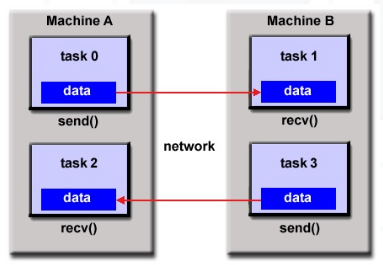
\includegraphics[width=0.7\linewidth]{img/modello-trasmissione-messaggi}
	\caption{modello di trasmissione dei messaggi.}
	\label{fig:modello-trasmissione-messaggi}
\end{figure}
Il modello di trasmissione dei messaggi (figura \ref{fig:modello-trasmissione-messaggi}) dimostra le seguenti caratteristiche:
\begin{itemize}
	\item una serie di task che usano la propria memoria locale durante la computazione. Tasks multipli possono risiedere fisicamente sulla stessa macchina e su un numero arbitrario di macchine;
	\item i task comunicano attraverso l'invio e la ricezione di messaggi;
	\item il trasferimento dei messaggi di solito richiede l'esecuzione di operazioni cooperative da parte di ciascun processo. Ad esempio, un'operazione di invio deve avere un'operazione di ricezione corrispondente.
\end{itemize}

\subsubsection{Implementazione del modello di passaggio dei messaggi} Dal punto di vista della programmazione, le implementazioni dello scambio di messaggi comprendono comunemente una libreria di subroutine incorporate nel codice sorgente. Il programmatore è responsabile di tutto il parallelismo. Nel 1992 è stato formato il Forum MPI con l'obbiettivo primario di stabilire un'interfaccia standard per le implementazioni dello scambio di messaggi. MPI è ora lo standard industriale "de facto" per lo scambio di messaggi.

Per le architetture a memoria condivisa, le implementazioni MPI solitamente non utilizzano una rete per le comunicazioni delle attività. Usano la propria memoria condivisa per motivi di prestazioni.

\subsection{Modello data parallel}
\begin{figure}[th]
	\centering
	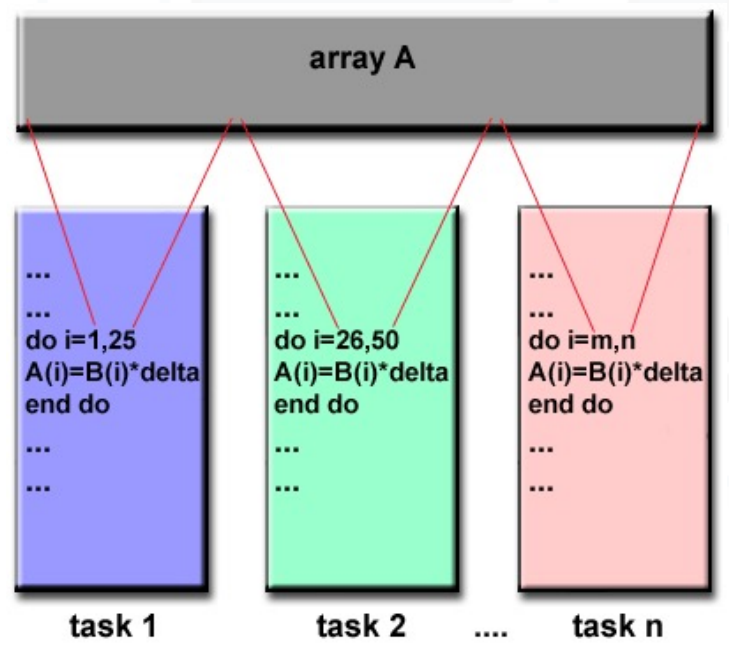
\includegraphics[width=0.7\linewidth]{img/modello-parallelo-dei-dati}
	\caption{modello data parallel.}
	\label{fig:modello-parallelo-dei-dati}
\end{figure}
Il modello data parallel (figura \ref{fig:modello-parallelo-dei-dati}) ha le seguenti caratteristiche:
\begin{itemize}
	\item la maggior parte del lavoro si concentra sull'esecuzione di operazioni su un set di dati. Il set è generalmente organizzato in una \textbf{struttura  dati comune}, ad esempio un array o un cubo;
	\item una serie di attività lavora collettivamente sulla stessa struttura dati, tuttavia, ogni attività funziona su una partizione diversa della stessa struttura dati;
	\item le attività eseguono la stessa operazione sulla loro partizione di lavoro, ad esempio "aggiungi 4 a ogni elemento dell'array";
	\item nelle architetture a memoria condivisa, tutte le attività possono avere accesso alla struttura dei dati attraverso la memoria globale. Nelle architetture di memoria distribuita la struttura dei dati è suddivisa e risiede come "chunks" (ovvero "pezzi") nella memoria locale di ciascun task.
\end{itemize}

\subsubsection{Implementazione del modello data parallel} La programmazione con il modello data parallel viene solitamente compiuta scrivendo un programma con costrutti data parallel. I costrutti possono essere chiamati tramite subroutine di una libreria che supporta data parallel o attraverso direttive per un compilatore data parallel.

Le implementazioni più comuni sono:
\begin{itemize}
	\item HPF (High Performance Fortran);
	\item direttive di compilatore;
\end{itemize}

\subsection{Modello ibrido} È un modello in cui possono essere combinati due o più modelli di programmazione parallela. Un esempio comune è di combinare il MPI (Message Passing Model) con il modello delle thread (thread POSIX) o in alternativa il modello della memoria condivisa (OpenMP).

Un altro esempio comune di modello ibrido consiste nel combinare i dati in parallelo con lo scambio di messaggi.
\subsection{Modello SPMD (Single Program Multiple Data)} SPMD è in realtà un modello di programmazione di "alto livello" che può essere costruito su qualsiasi combinazione dei modelli di programmazione parallela precedentemente menzionati. Un singolo programma viene eseguito da tutti i task contemporaneamente. In qualsiasi momento, le attività possono eseguire le stesse o differenti istruzioni all'interno dello stesso programma (figura \ref{fig:spmd}).
\begin{figure}[th]
	\centering
	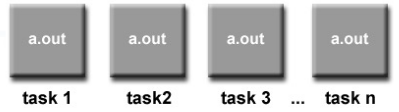
\includegraphics[width=0.7\linewidth]{img/SPMD}
	\caption{modello SPMD.}
	\label{fig:spmd}
\end{figure}
A differenza di SIMD (Single Instruction Multiple Data), nel SPMD, più processori autonomi eseguono simultaneamente lo stesso programma in punti indipendenti, anziché in unico \textbf{lockstep} che SIMD